
\chapter[Tópicos de Gerenciamento de Requisitos]{Tópicos de Gerenciamento de Requisitos}
\section{Rastreabilidade de Requisitos}
A Rastreabilidade de Requisitos (descrever, mostrar e acompanhar a vida de um requisito nos sentidos \emph{forward-to} e \emph{forward-from} \cite{garcia001}) é tido como uma das soluções para o problema da dessincronização entre \emph{software} e seus requisitos, sendo que a solução desse problema é quase que uma exigência básica da industria de desenvolvimento de \emph{software} atual \cite{leal001}. Faz parte de uma \emph{Specific Practice} da área de processo \emph{Requirements Management} do CMMI. É divida entre \emph{forward-to} (itens que derivam de um requisito \emph{x}) e \emph{forward-from} (itens que são derivados de um requisito \emph{x}).

Evidentemente que a Rastreabilidade de Requisitos muda de abordagem para abordagem. Será mostrada então o formato de rastreabilidade do grupo 1, levando em consideração que o framework de abordagem utilizado é o SAFe.

Primeiro, é lembrado que do tema de investimento será derivado o épico. Um épico pode ser classificado em arquitetural ou de negócio, e dele derivarão \emph{features}. Das \emph{features} serão derivadas estórias de usuário, que delas (as estórias de usuário) derivam tarefas e, no nosso contexto, testes funcionais.

A nomenclatura utilizada será uma concatenação entre prefixo (mostrados abaixos) e sufixos (número do índice do item). Lista de prefixos utilizados:

\begin{tabular}{c | c | c}
  \hline
  Item & Prefixo & Prefixo+sufixo (exemplo)\\ \hline
  Tema de Investimento & IT & IT0004 \\
  Epico & EP & EP0002 \\
  Feature & FE & FE0033 \\
  Estória de Usuário & US & US0243 \\
  Tarefas & TS & TS0932 \\
  Teste Funcional & FT & FT2142 \\
  \hline
\end{tabular}

\newpage
Esquema da rastreabilidade:

\begin{figure}[h]
  \centering
  \caption{Esquema de rastreabilidade de requisitos que será utilizado}
  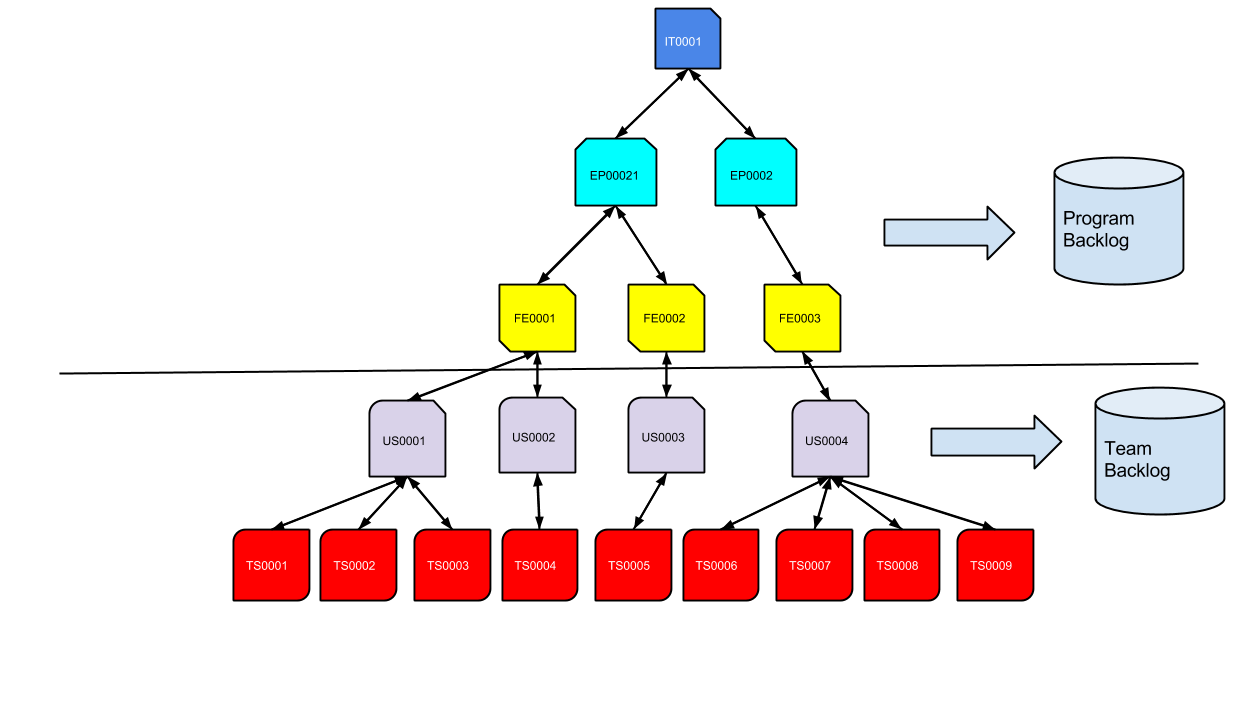
\includegraphics[scale=0.4]{figuras/Matriz.ps}
\end{figure}

\section{Atributos de Requisitos}
Requisitos, assim como objetos do mundo real, possuem atributos que os descrevem. Um carro, por exemplo, tem determinada potência, consome determinada quantidade de combustível, etc. Os requisitos são da mesma forma: apresentam atributos que os descrevem \cite{tel006}.

Existem diversas maneiras de se analisar qual requisito deve receber maior prioridade, e isso quase sempre é feito levando em consideração seus atributos. No contexto deste projeto, será utilizado o \emph{High Delay Cost First} em conjunto com o \emph{WSJF - Weighted Shortest Job First}, também sugerido por \cite{safe001}. O \emph{High Delay Cost First} consiste em se dar prioridade as \emph{features} que apresentam maior penalização a cada atraso, enquanto o \emph{WSJF} consiste em se dar prioridade as \emph{features} que necessitam de menos esforço, mas que punem maior a cada atraso. Os dois se complementam, e no final das contas se faz a feature com o maior \emph{weight} (peso), que é dado pela fórmula \emph{Peso = Custo do atraso / Esforço} \cite[p. 266]{safe001}.

Ou seja, devemos ter como atributos de requisitos pelo menos os necessários para utilizar o HDCF e o WSJF. Eles são: \emph{esforço, dificuldade, custo, tempo, prioridade}. Mas, em conjunto, também utilizaremos alguns atributos sugeridos por \cite{tel006}.

Sendo assim, os atributos de requisitos utilizados pelo grupo 1 serão:
\begin{itemize}
  \item Fonte: De onde este requisito é derivado? Pessoa, documento, outro requisito, etc.
  \item Prioridade: Este requisito tem prioridade alta, média ou baixa?
  \item Comentários: Comentários de quem documentou tal requisito.
  \item Status: Condição atual do requisito (concluído, não começado, ou em progresso).
  \item Risco: Qual o risco de determinado requisito durante sua implantação? Podendo ser alto, médio ou baixo.
  \item Prazo: Até quando tal requisito deve estar pronto?
  \item Nível de teste: Qual o nível de teste de determinado requisito? Poderá ser nulo, médio, ou suficiente.
  \item Esforço: Quanto esforço é necessário para se concluir determinado requisito? Poderá ser alto, médio ou baixo.
  \item Custo do atraso: Quão grande é a punição por atraso de determinado requisito? Poderá ser alto, médio ou baixo.
\end{itemize}

Na fórmula citada acima (WSJF), será assumido valor 3 para alto, 2 para médio e 1 para baixo para os atributos correspodentes. Exemplo: Um requisito com custo do atraso alto e esforço médio:

\begin{equation}
  Peso = C / E = 3/2 = 1.5
\end{equation}
  \emph{Onde: C = Custo do atraso, E = Esforço.}

Contra um requisito com custo do atraso baixo e esforço alto:

\begin{equation}
  Peso = 1/3 = 0.3333
\end{equation}

Nesse caso, o primeiro requisito seria implementado primeiro, pois apresenta maior peso.
